\chapter{Analiza danych oraz test algorytmów}
\label{cha:analizaDanych}

Prace nad systemem kategoryzacji zacząłem od wyboru danych na których będę bazował. Wybór padł na dane z obszaru newsów - jego motywacją był jasny podział na kategorie. Niemal w każdym przypadku człowiek jest w stanie odróżnić wiadomość sportową od wiadomości ze świata biznesu. Dodatkowym atutem była jakość danych znajdujących się w internecie. Każdy news ze znanych portali informacyjnych ma jasno przypisaną kategorię oraz zazwyczaj jego zawartość jest dobrej jakości - nie zawiera kolokwialnego języka, błędów ortograficznych oraz literówek, które utrudniałyby jego przetwarzanie. Dla ułatwienia projektu skupiłem się na danych w języku angielskim - z powodu jego popularności jest on obecnie językiem, który najłatwiej poddaje się przetwarzaniu maszynowemu.

Po wstępnym zebraniu danych zamierzałem wyciągnąć z nich informacje stosując następujące kroki:

\begin{enumerate}
    \item Wstępne przetworzenie danych tekstowych.
    \item Sprowadzenie ich do modelu Bag Of Words oraz TF-IDF.
    \item Podzielenie danych na zbiór uczący i testowy.
    \item Sprawdzenie skuteczności różnych algorytmów nadzorowanego uczenia maszynowego na zebranych danych.
\end{enumerate}

%---------------------------------------------------------------------------

\section{Gromadzenie danych}
\label{sec:gromadzenieDanych}

Pierwszy zestaw newsów do analizy pochodził ze źródła www.inshorts.com, w którym możemy znaleźć wiadomości z różnych kategorii z których każdy ma długość około 60 słów. Struktura pobranych danych składała się z dwóch elementów - zawartości newsa (content) oraz etykiety opisującej go (label).

    \begin{figure}[H]
    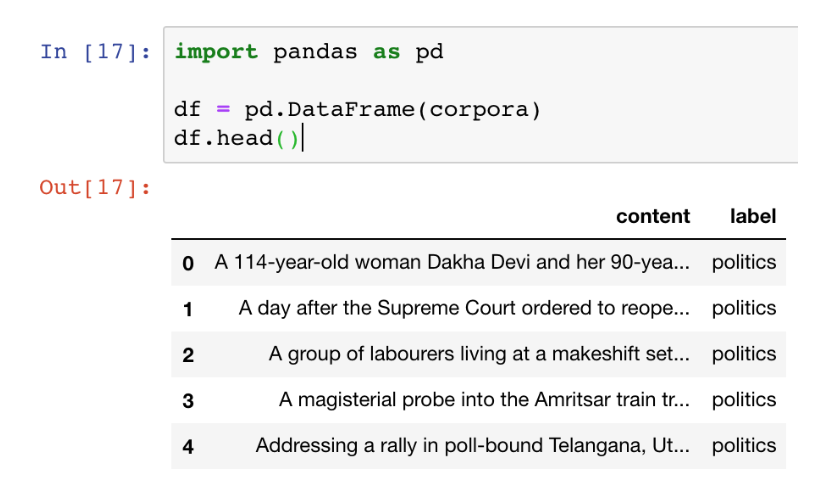
\includegraphics[width=8cm]{content_example.png}
    \centering
    \caption{Przykład zebranych danych.}
    \end{figure} 
    
Histogram ilości słów dla 2657 newsów:

    \begin{figure}[H]
    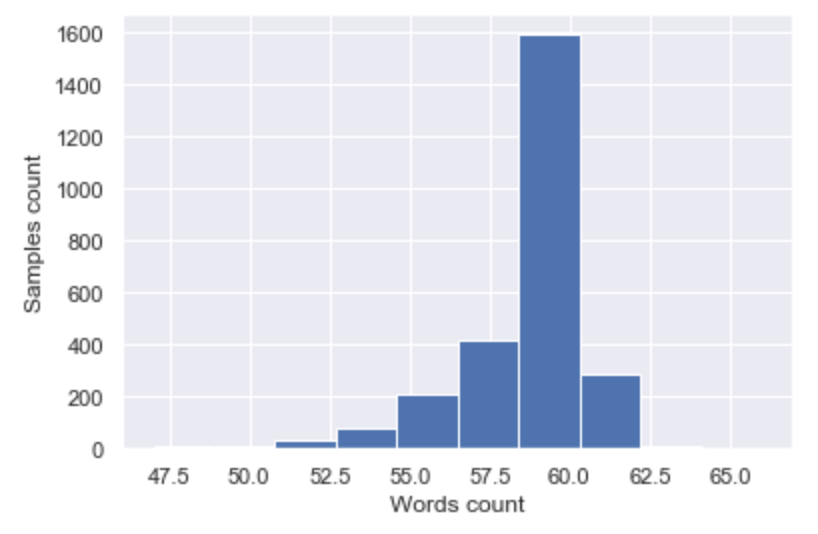
\includegraphics[width=8cm]{words_count.png}
    \centering
    \caption{Histogram ilości słów w tekście}
    \end{figure} 

\section{Wstępne przetwarzanie danych}

Surowe dane tekstowe pobrane z internetu nie do końca nadają się do użycia w algorytmach uczenia maszynowego. Zawierają one znaki interpunkcyjne, duże litery, stop-słowa \footnote{https://www.seopilot.pl/wiki/Stopwords.html} oraz te same wyrazy w różnej formie gramatycznej. Aby ułatwić analizę danych oraz uczenie algorytmów zastosowałem kilka kroków przetwarzania wstępnego danych w celu ich uproszczenia:

\begin{enumerate}
    \item Zamiana wielkich liter na małe.
    \item Usunięcie znaków interpunkcyjnych oraz cyfr.
    \item Zamiana wszystkich znaków na znaki występujące w zbiorze ASCII.
    \item Lematyzacja, czyli sprowadzenie słów do ich podstawowych form gramatycznych.
    \item Usunięcie stop-słów.
\end{enumerate}

\newpage
Przykładowy tekst przed i po przetworzeniu:

\begin{verbatim}
    TEKST WEJŚCIOWY: 
    There’s been a lot written about the theory behind TF-IDF but the 
    gist is: calculate the term frequency (TF), or number of times 
    a word appears across the text you’re interested in analysing.
    This is intuitive - more important words appear 
    more often right?
    
    TEKST WYJŚCIOWY: 
    lot written theory behind tfidf gist calculate term frequency
    tf number time word appears across text youre interested
    analysing intuitive important word appear often right
\end{verbatim}

Aby lepiej zrozumieć istotę przetwarzania wstępnego danych tekstowych, na wykresie \ref{wykr:slowa_bez_pre} widać 10 najczęściej występujących słów we wszystkich zebranych newsach. Są to głównie słowa nie niosące za sobą konkretnej informacji, które mogą wpływać negatywnie na sprawność algorytmów uczenia maszynowego. 

    \begin{figure}[H]
    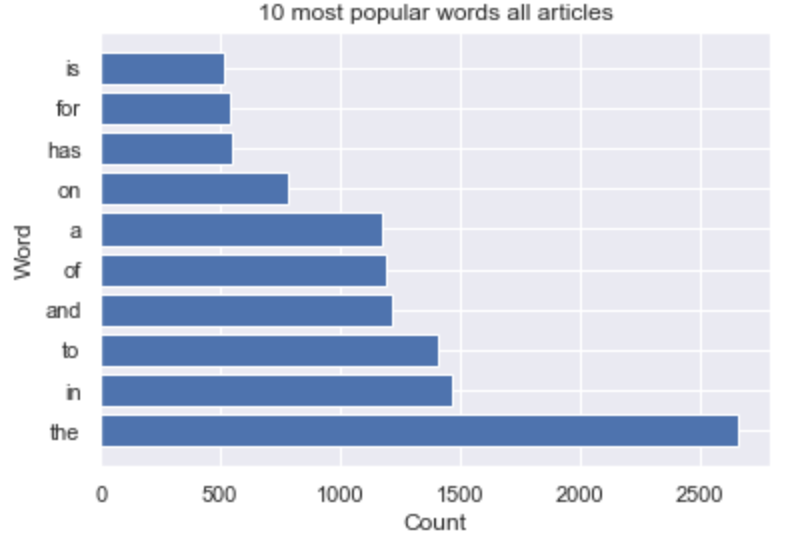
\includegraphics[width=8cm]{images/analiza/all_unprocessed.png}
    \centering
    \caption{10 najpopularniejszych słów w całym korpusie bez zastosowania wstępnego przetwarzania.}
    \label{wykr:slowa_bez_pre}
    \end{figure} 

\section{Wizualizacja danych}

Po przetworzeniu tekstu możemy go poddać analizie częstotliwości występowania słów w każdej kategorii. Na wykresach \ref{fig:10_most_popular_words} widać wyraźnie, że zestawy słów różnią się pomiędzy sobą. Słowa które się powtarzają to są czasownikami charakterystycznymi dla newsów (said, have, was itp.). Z występowania tych słów również można wyciągnąć ciekawe wnioski. Na przykład duża popularność słowa 'said' w kategorii rozrywka może świadczyć o dużej ilości cytatów w artykułach z tej kategorii.

\begin{figure}[H]
     \centering
     \begin{subfigure}[b]{0.7\textwidth}
         \centering
         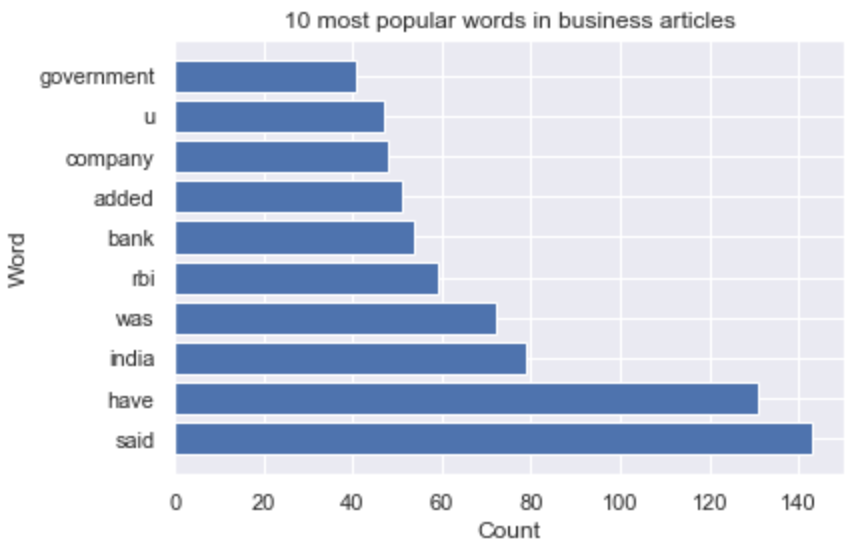
\includegraphics[width=\textwidth]{images/analiza/business.png}
     \end{subfigure}
     \hfill
     \begin{subfigure}[b]{0.7\textwidth}
         \centering
         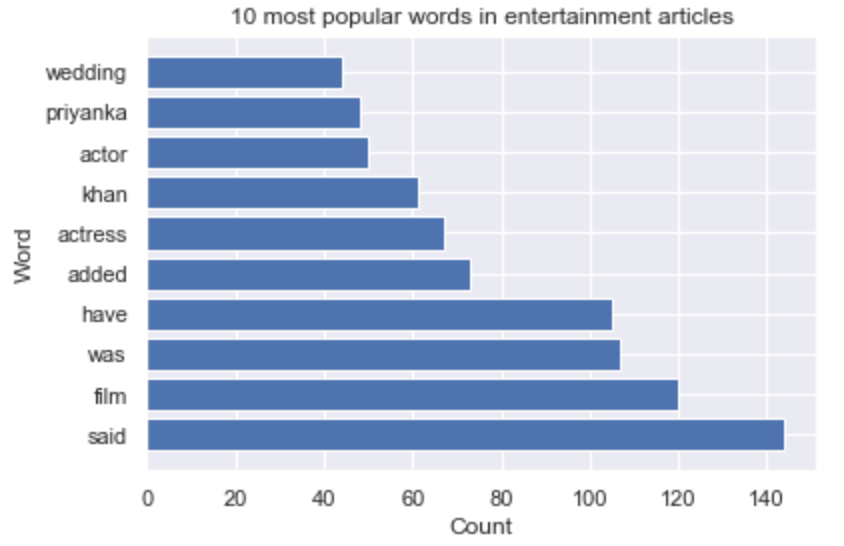
\includegraphics[width=\textwidth]{images/analiza/entertainment.png}
     \end{subfigure}
     \hfill
     \begin{subfigure}[b]{0.7\textwidth}
         \centering
         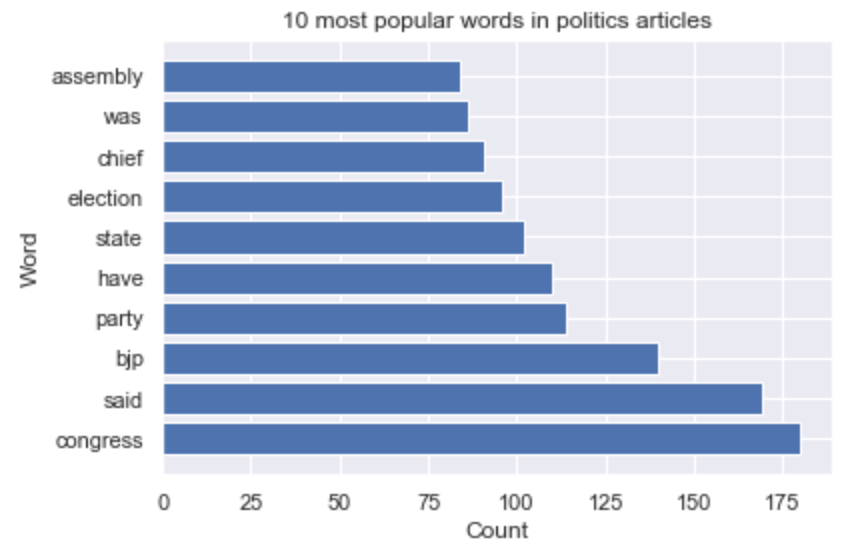
\includegraphics[width=\textwidth]{images/analiza/politics.png}
     \end{subfigure}
\end{figure}
\begin{figure}[H]\ContinuedFloat                 \begin{subfigure}[b]{0.7\textwidth}
         \centering
         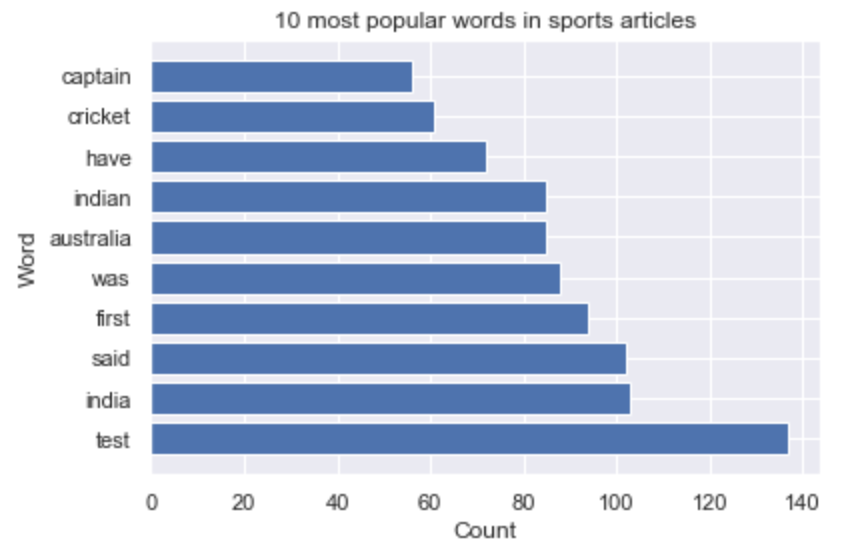
\includegraphics[width=\textwidth]{images/analiza/sports.png}
     \end{subfigure}
     \hfill
     \begin{subfigure}[b]{0.7\textwidth}
         \centering
         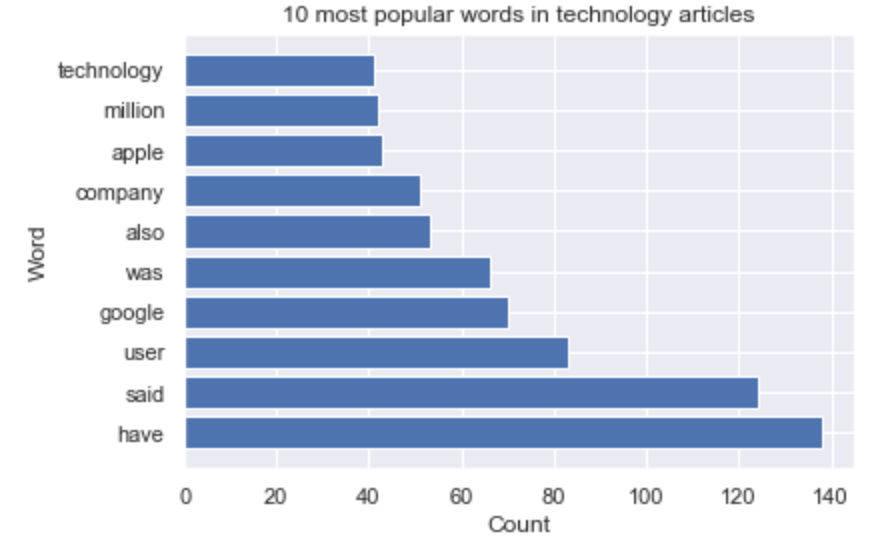
\includegraphics[width=\textwidth]{images/analiza/technology.png}
     \end{subfigure}
        \caption{Najpopularniejsze wyrazy w każdej z analizowanych kategorii}
        \label{fig:10_most_popular_words}
\end{figure}

\newpage
\newpage
Kolejnym analizowanym aspektem są bi-gramy, czyli częstotliwość występowania dwóch słów obok siebie. Na podstawie zebranych danych wygląda to następująco:

\begin{figure}[H]
     \centering
     \begin{subfigure}[b]{0.7\textwidth}
         \centering
         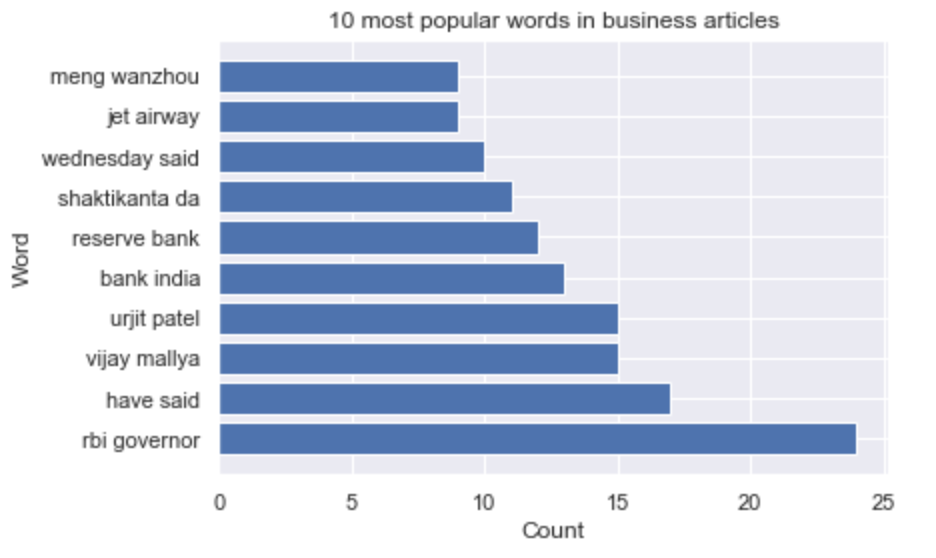
\includegraphics[width=\textwidth]{images/analiza/business_bigram.png}
     \end{subfigure}
     \hfill
     \begin{subfigure}[b]{0.7\textwidth}
         \centering
         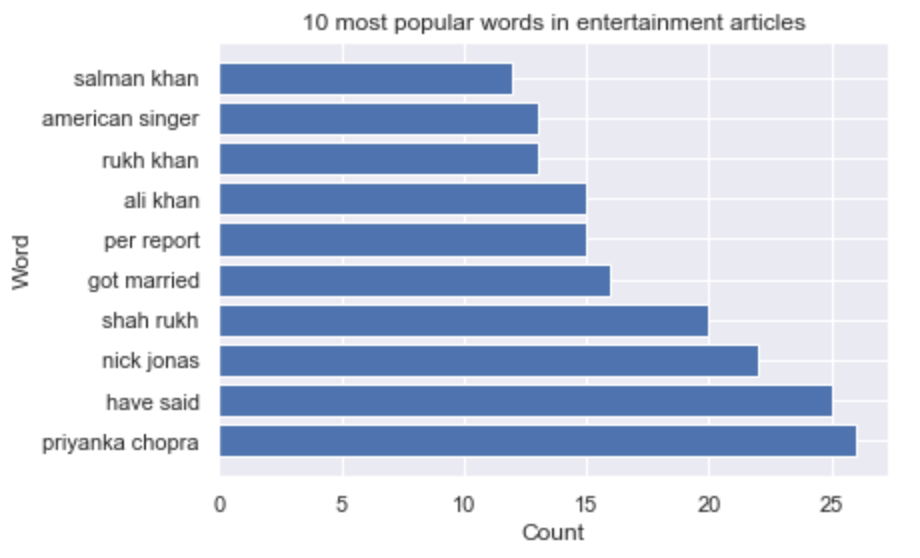
\includegraphics[width=\textwidth]{images/analiza/entertainment_bigram.png}
     \end{subfigure}
     \hfill
     \begin{subfigure}[b]{0.7\textwidth}
         \centering
         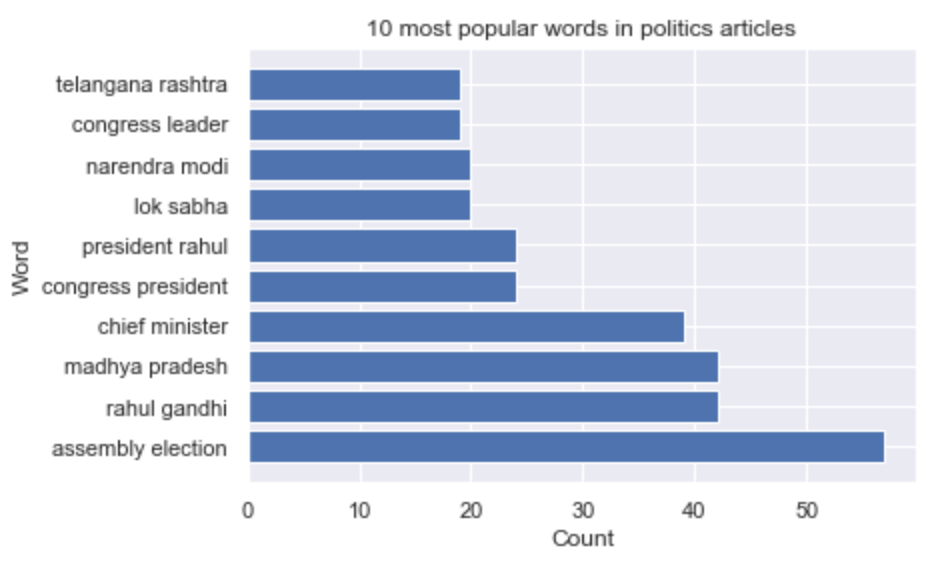
\includegraphics[width=\textwidth]{images/analiza/politics_bigram.png}
     \end{subfigure}
\end{figure}
\begin{figure}[H]\ContinuedFloat
     \begin{subfigure}[b]{0.7\textwidth}
         \centering
         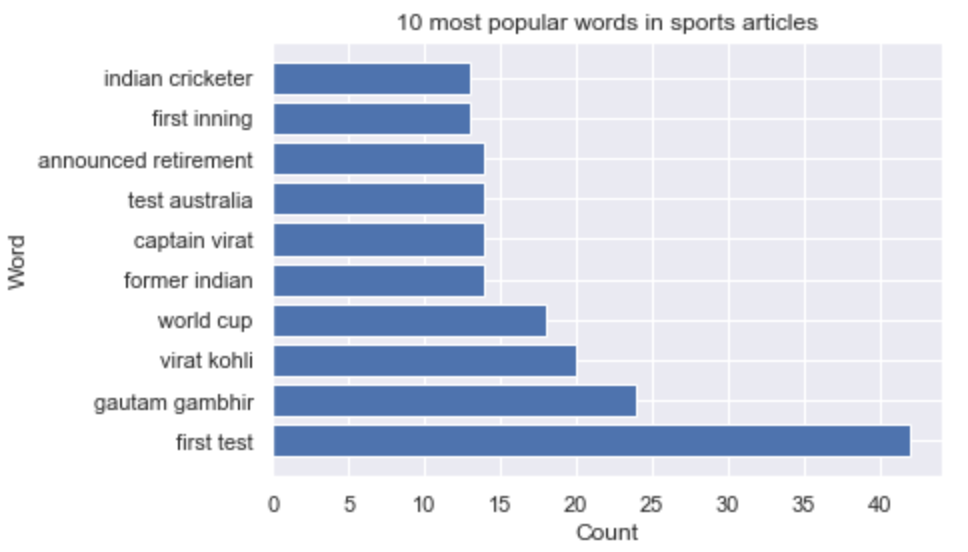
\includegraphics[width=\textwidth]{images/analiza/sports_bigram.png}
     \end{subfigure}
     \hfill
     \begin{subfigure}[b]{0.7\textwidth}
         \centering
         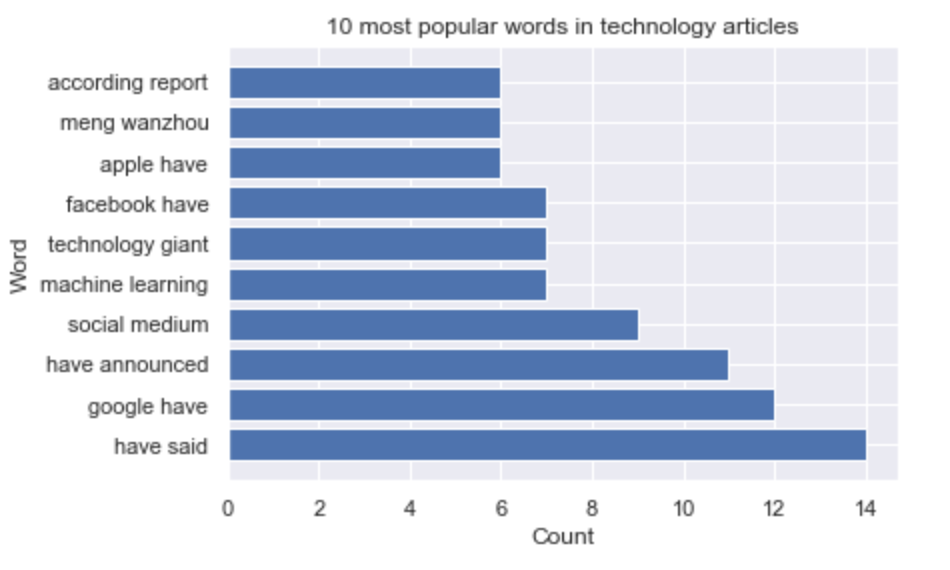
\includegraphics[width=\textwidth]{images/analiza/technology_bigram.png}
     \end{subfigure}
        \caption{Najpopularniejsze 2-gramy w każdej z analizowanych kategorii}
        \label{fig:10_most_popular_ngrams}
\end{figure}

Pojawiło się tutaj pewne zakłócenie - z racji, że dane pochodzą z jednego źródła pojawiło się kilka imion i nazwisk osób oraz nazw własnych. Jednak jest też kilka ciekawych pozycji takich jak 'have announced' w kategorii artykułów technologicznych, czy 'assembly election' dotyczących polityki. Prawdopodobnie przy zaczerpnięciu danych z większej ilości źródeł wyniki byłyby dużo bardziej satysfakcjonujące.

\newpage
\section{Test klasyfikatorów}

W celu wybrania najlepszych klasyfikatorów wybrałem dwa modele przetworzenia danych: bag of words oraz term frequency - inverse document frequency. Dane zostały podzielone na zbiór treningowy oraz testowy w stosunku 8:2. Wyniki testu znajdują się na poniższym wykresie. Przedstawiają one uzyskaną skutecznośc algorytmu, czyli jaka część danych ze zbioru testowego została poprawnie sklasyfikowana.

\begin{figure}[H]
     \centering
     \begin{subfigure}[b]{0.8\textwidth}
         \centering
         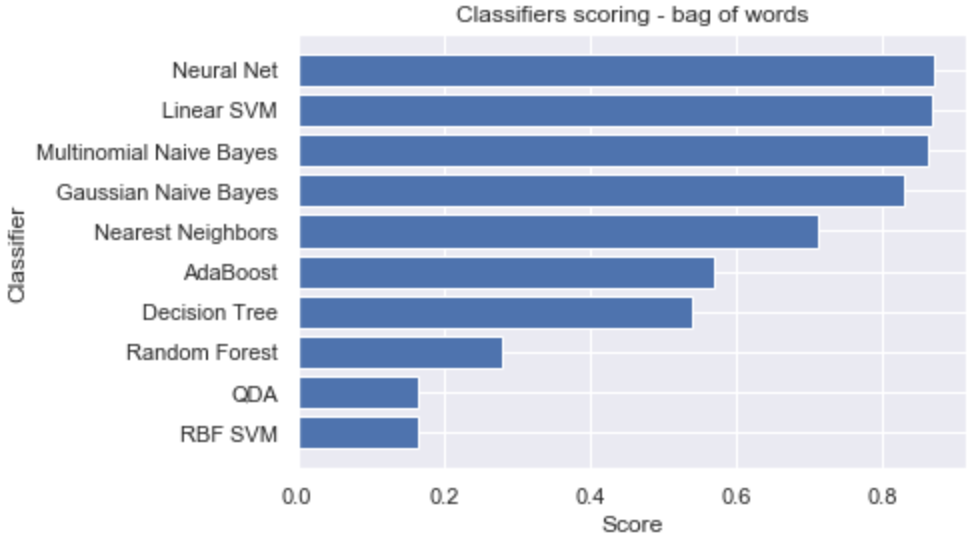
\includegraphics[width=\textwidth]{images/analiza/classifiers_bag.png}
     \end{subfigure}
     \hfill
     \begin{subfigure}[b]{0.8\textwidth}
         \centering
         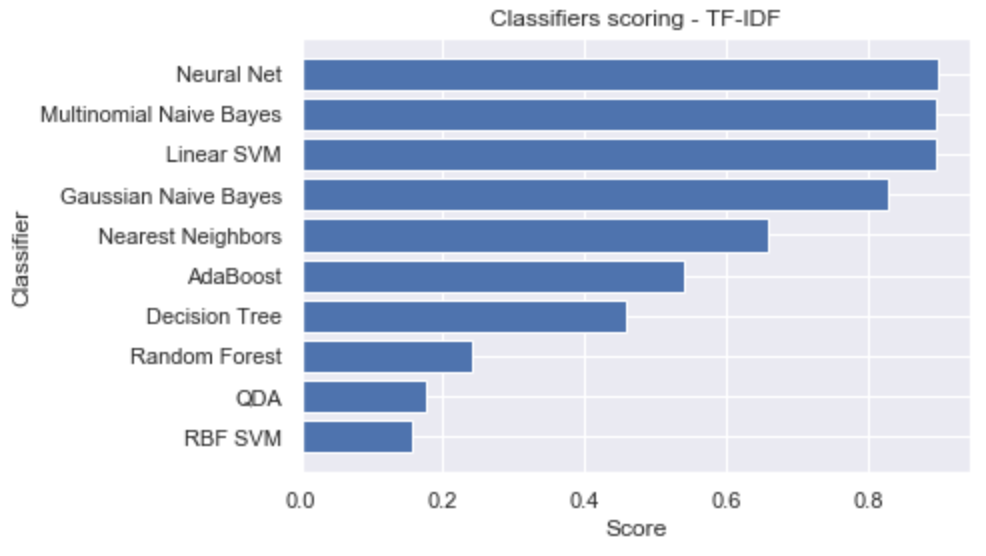
\includegraphics[width=\textwidth]{images/analiza/classifiers_tfidf.png}
     \end{subfigure}
        \caption{Skuteczność różnych klasyfikatorów}
        \label{fig:classifiers_test}
\end{figure}

Z tego badania można wywnioskować, że użyty model danych (bag of words/TF-IDF) nie miał znaczącego wpływu na skuteczność algorytmów uczenia nadzorowanego. W obu przypadkach obiecujące wyniki uzyskały trzy algorytmy:
\begin{enumerate}
    \item Sieć neuronowa.
    \item Liniowa maszyna wektorów nośnych.
    \item Naiwny klasyfikator bayesowski (w dwóch wariacjach).
\end{enumerate}

\section{Klasteryzacja}

W ramach przeprowadzanych doświadczeń, postanowiłem również sprawdzić jak zebrane dane będą podatne na uczenie nienadzorowane. Badania rozpocząłem od użycia algorytmu k-średnich (ang. k-means) na przetworzonych danych i próbie podzielenia ich na klastry.

Do walidacji rezultatów wykorzystałem kategorie przypisane do danych. Dla idealnie działającego algorytmu klasteryzacji jedna kategoria powinna występować tylko w jednym klastrze. Początkowo wykonałem dzielenie danych na dwa klastry - przeprowadziłem ten zabieg dwa razy (raz dla danych w formie Bag of Words, a raz jako TF-IDF).

    \begin{figure}[H]
    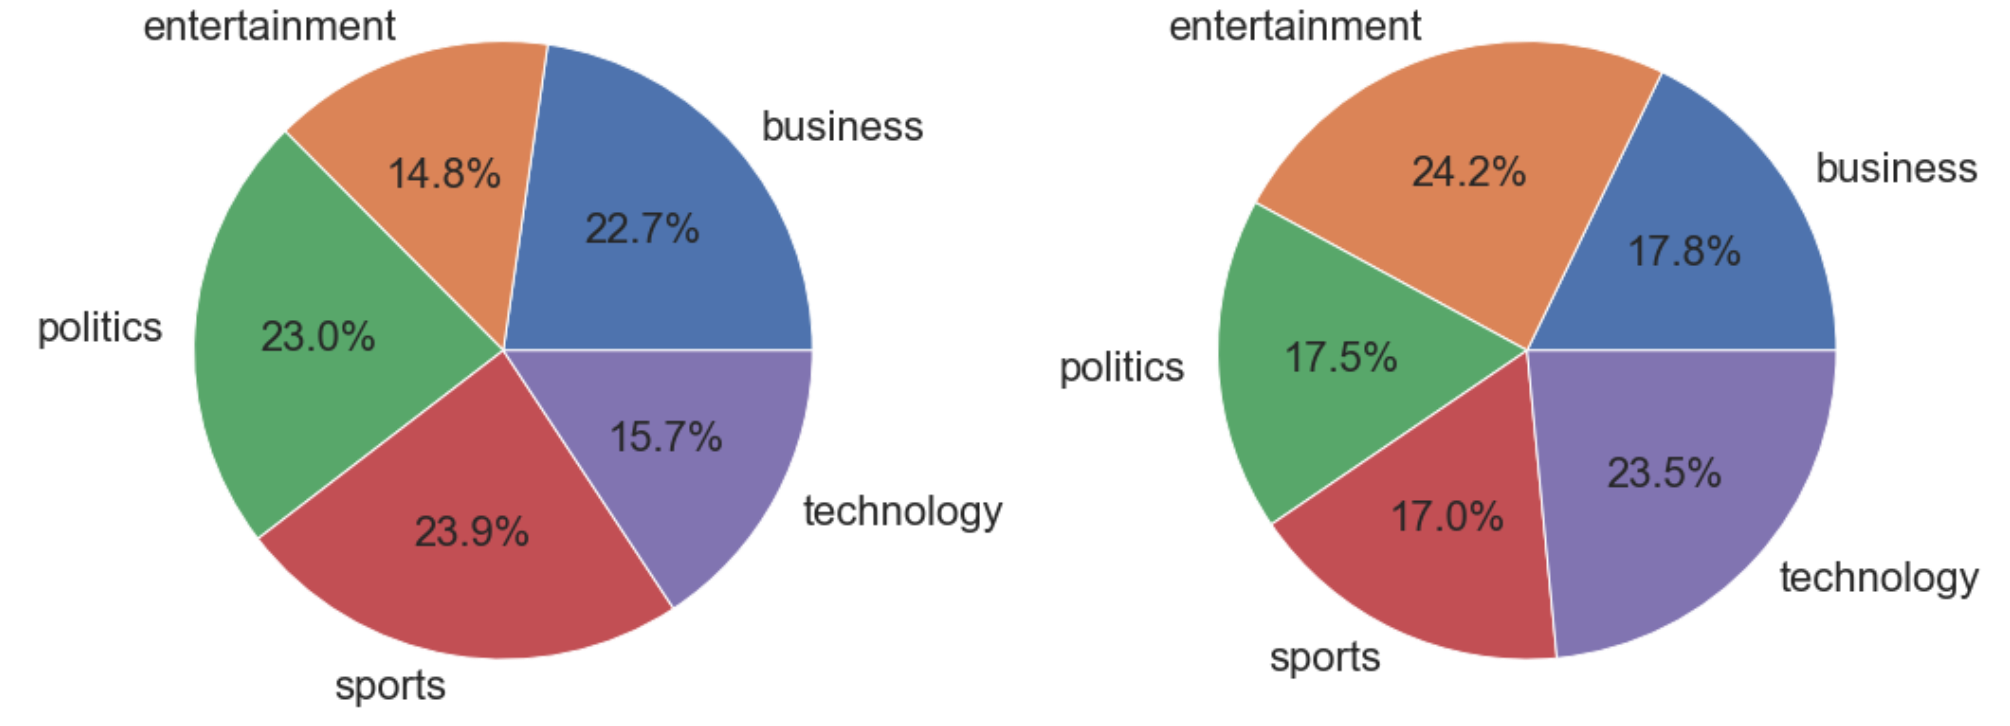
\includegraphics[width=\textwidth]{images/analiza/klast_bow.png}
    \centering
    \caption{Dwa klastry uzyskane z modelu Bag of Words}
    \label{fig:cls1}
    \end{figure} 
    
    \begin{figure}[H]
    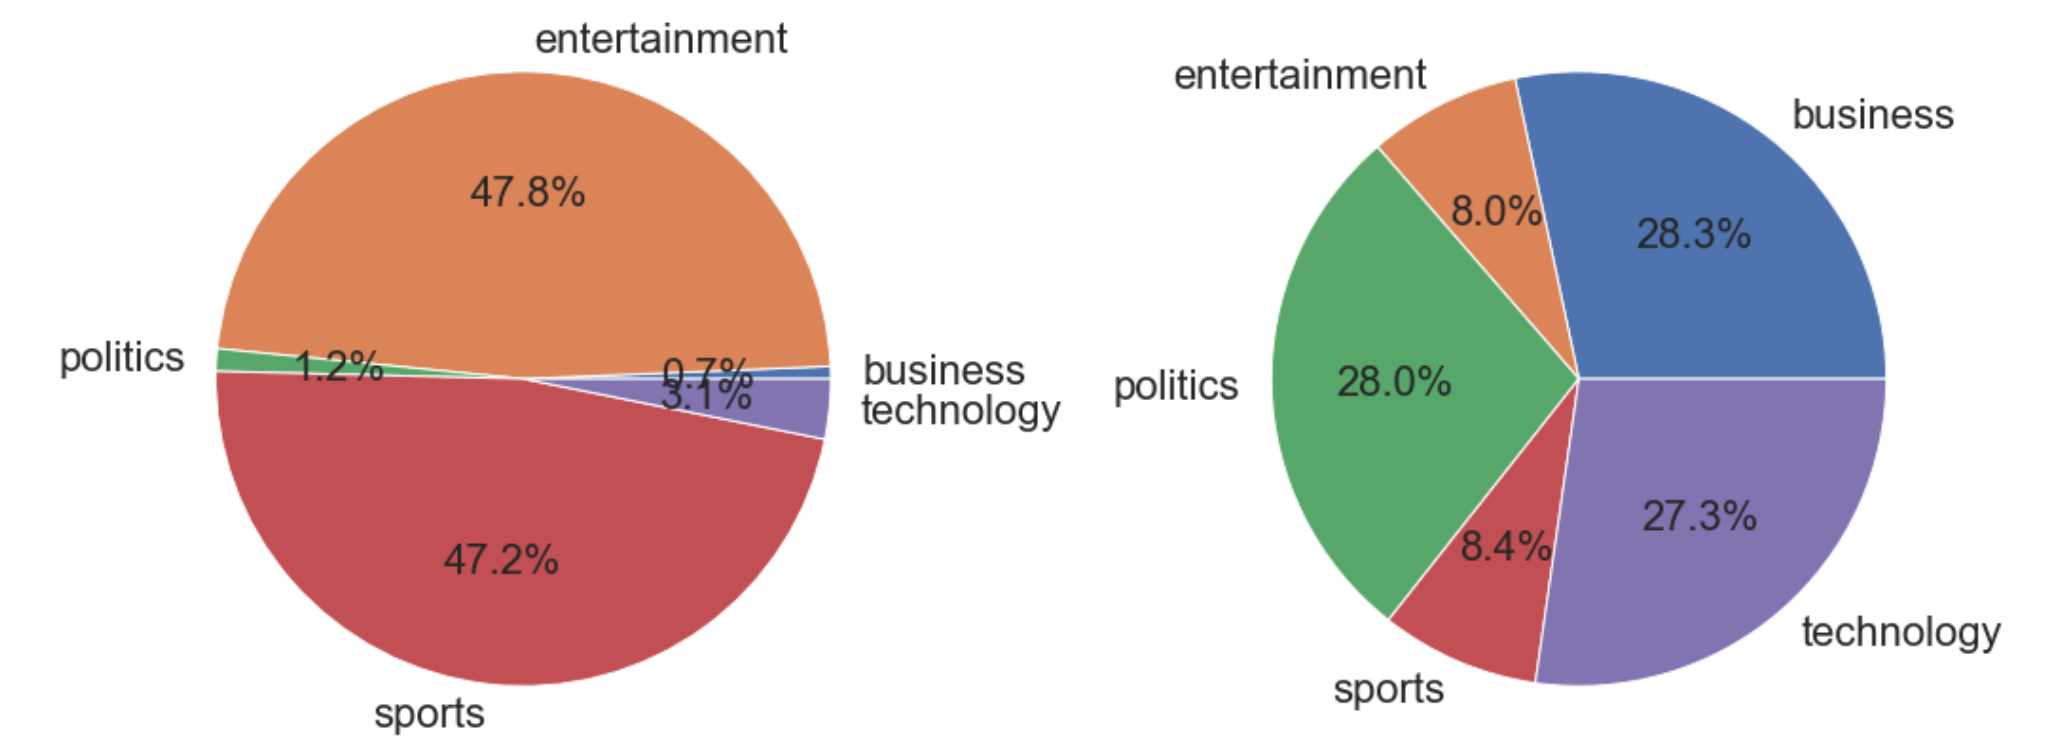
\includegraphics[width=\textwidth]{images/analiza/klast_tfidf.png}
    \centering
    \caption{2 klastry uzyskane z modelu TF-IDF}
        \label{fig:cls2}
    \end{figure} 

Na rysunku \ref{fig:cls2} widać wyraźne oddzielenie kategorii sport i rozrywka od reszty danych. Wskazuje to na fakt, że model TF-IDF wykazuje większą podatność na klasteryzację niż klasyczny Bag of Words. Dalsze próby będą kontynuowane bazując jedynie na danych TF-IDF.

W kolejnej próbie dane zostały podzielone na 5 klastrów, czyli tyle ile jest kategorii, którymi dane są oznaczone. Wizualizacja przedstawiona jest w odwrotnej formie - każdy wykres reprezentuje jedną kategorię i zawiera numery klastrów do których trafiły artykuły do niej należące.

\begin{figure}[H]
     \centering
     \begin{subfigure}[b]{0.38\textwidth}
         \centering
         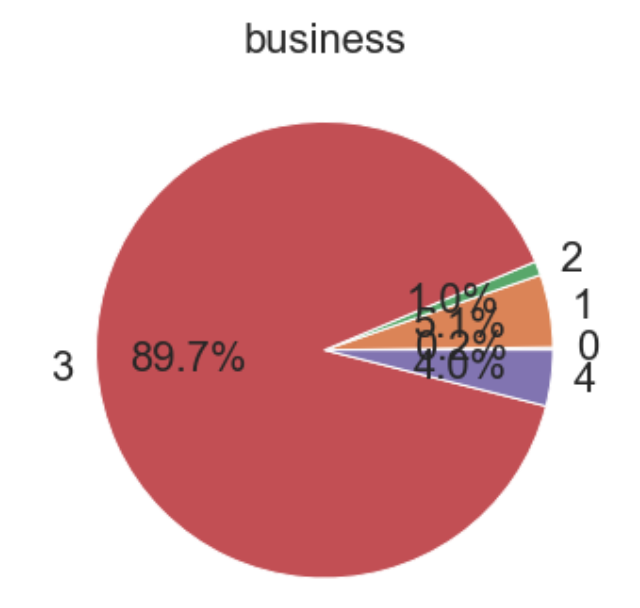
\includegraphics[width=\textwidth]{images/analiza/c_b.png}
     \end{subfigure}
     \hfill
     \begin{subfigure}[b]{0.34\textwidth}
         \centering
         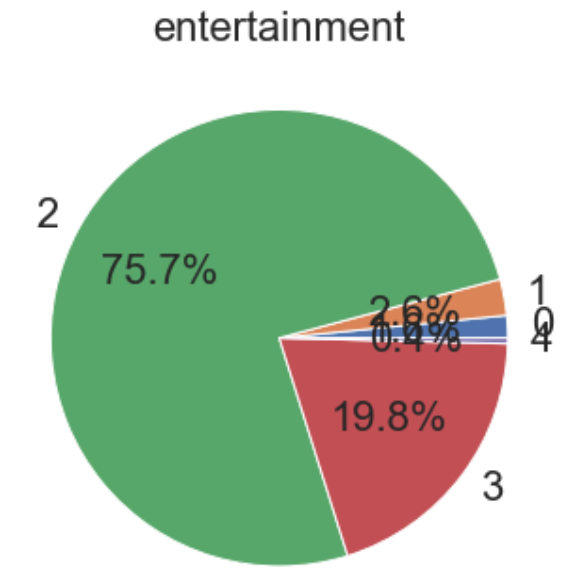
\includegraphics[width=\textwidth]{images/analiza/c_e.png}
     \end{subfigure}
     \hfill
     \begin{subfigure}[b]{0.38\textwidth}
         \centering
         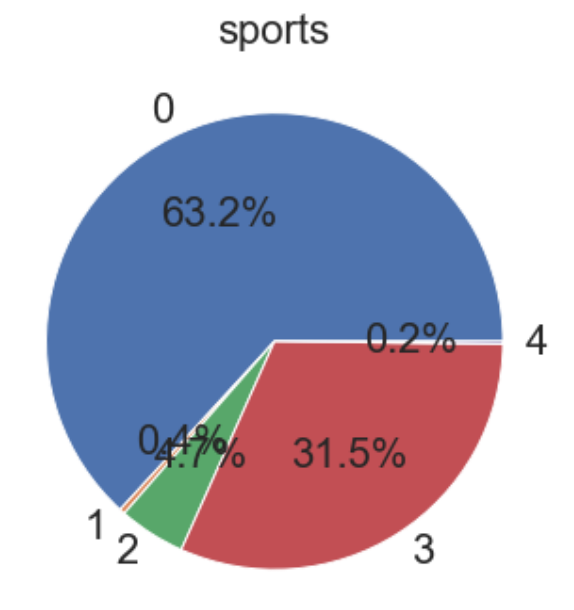
\includegraphics[width=\textwidth]{images/analiza/c_s.png}
     \end{subfigure}
     \hfill
     \begin{subfigure}[b]{0.38\textwidth}
         \centering
         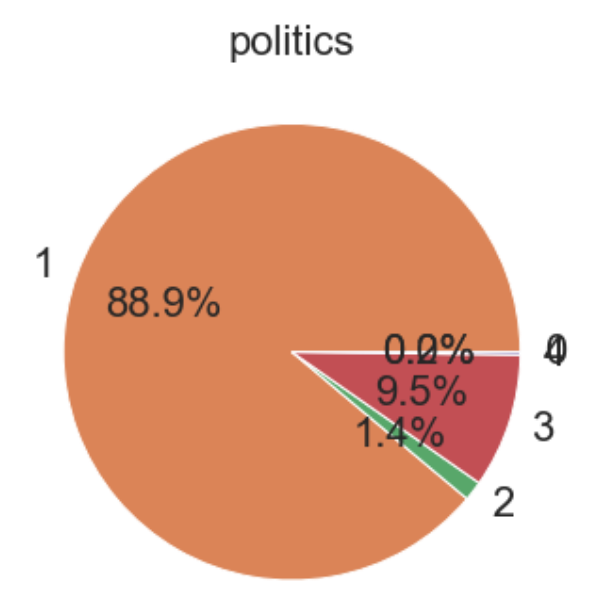
\includegraphics[width=\textwidth]{images/analiza/c_p.png}
     \end{subfigure}
     \hfill
     \begin{subfigure}[b]{0.38\textwidth}
         \centering
         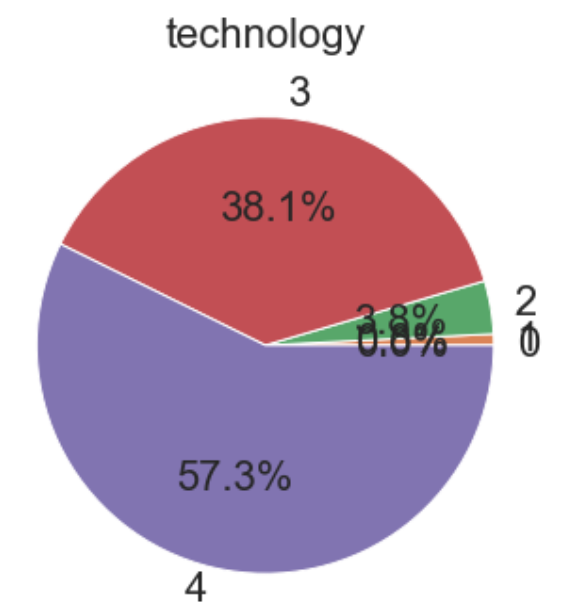
\includegraphics[width=\textwidth]{images/analiza/c_t.png}
     \end{subfigure}
        \caption{Rezultat podzielenia danych na 5 klastrów.}
        \label{fig:classifiers_test}
\end{figure}

Wyniki są zadowalające - artykuły rozrywkowe, technologiczne, polityczne i sportowe znalazły się w przeważającej mierze we własnych klastrach. Jedynie w klastrze 3, który zawiera w większości artykuły biznesowe znalazło się sporo artykułów o innej tematyce.

